\section{Product perspective}
\label{sec:product_perspective}%

\subsection{Class Diagrams}
\label{subsec:class_diagrams}%
The diagram below represents and describes the classes involved in the system, their basic functionalities, attributes,
and the relationships between them.
From the diagram, it is easy to see how the tournament entity function as a bridge between different
components. MOre specifically, in our design we assigned to this entity the task to hold track 
of battles, leaderboard of the tournament itself and badge assignment.
All the other functionalities are esily understandable from within the diagram or 
will be later discussed. \newline
Here, we want to stress that, even though just an high level view of the system-to-be, some consideration of implementation can be done. 
More specifically, some design pattern can be taken into consideration:
\begin{itemize}
    \item Decorator Pattern: to implement the logic behind the scoring system. Educator's choice of different aspect to consider will be easily managable 
    \item Observer patter: to implement the structure behind the notification system.
    \item Factory pattern: for the creation of different Badges with different characteristics and requirements.
  \end{itemize}

\begin{figure}[H]
    \begin{center}
        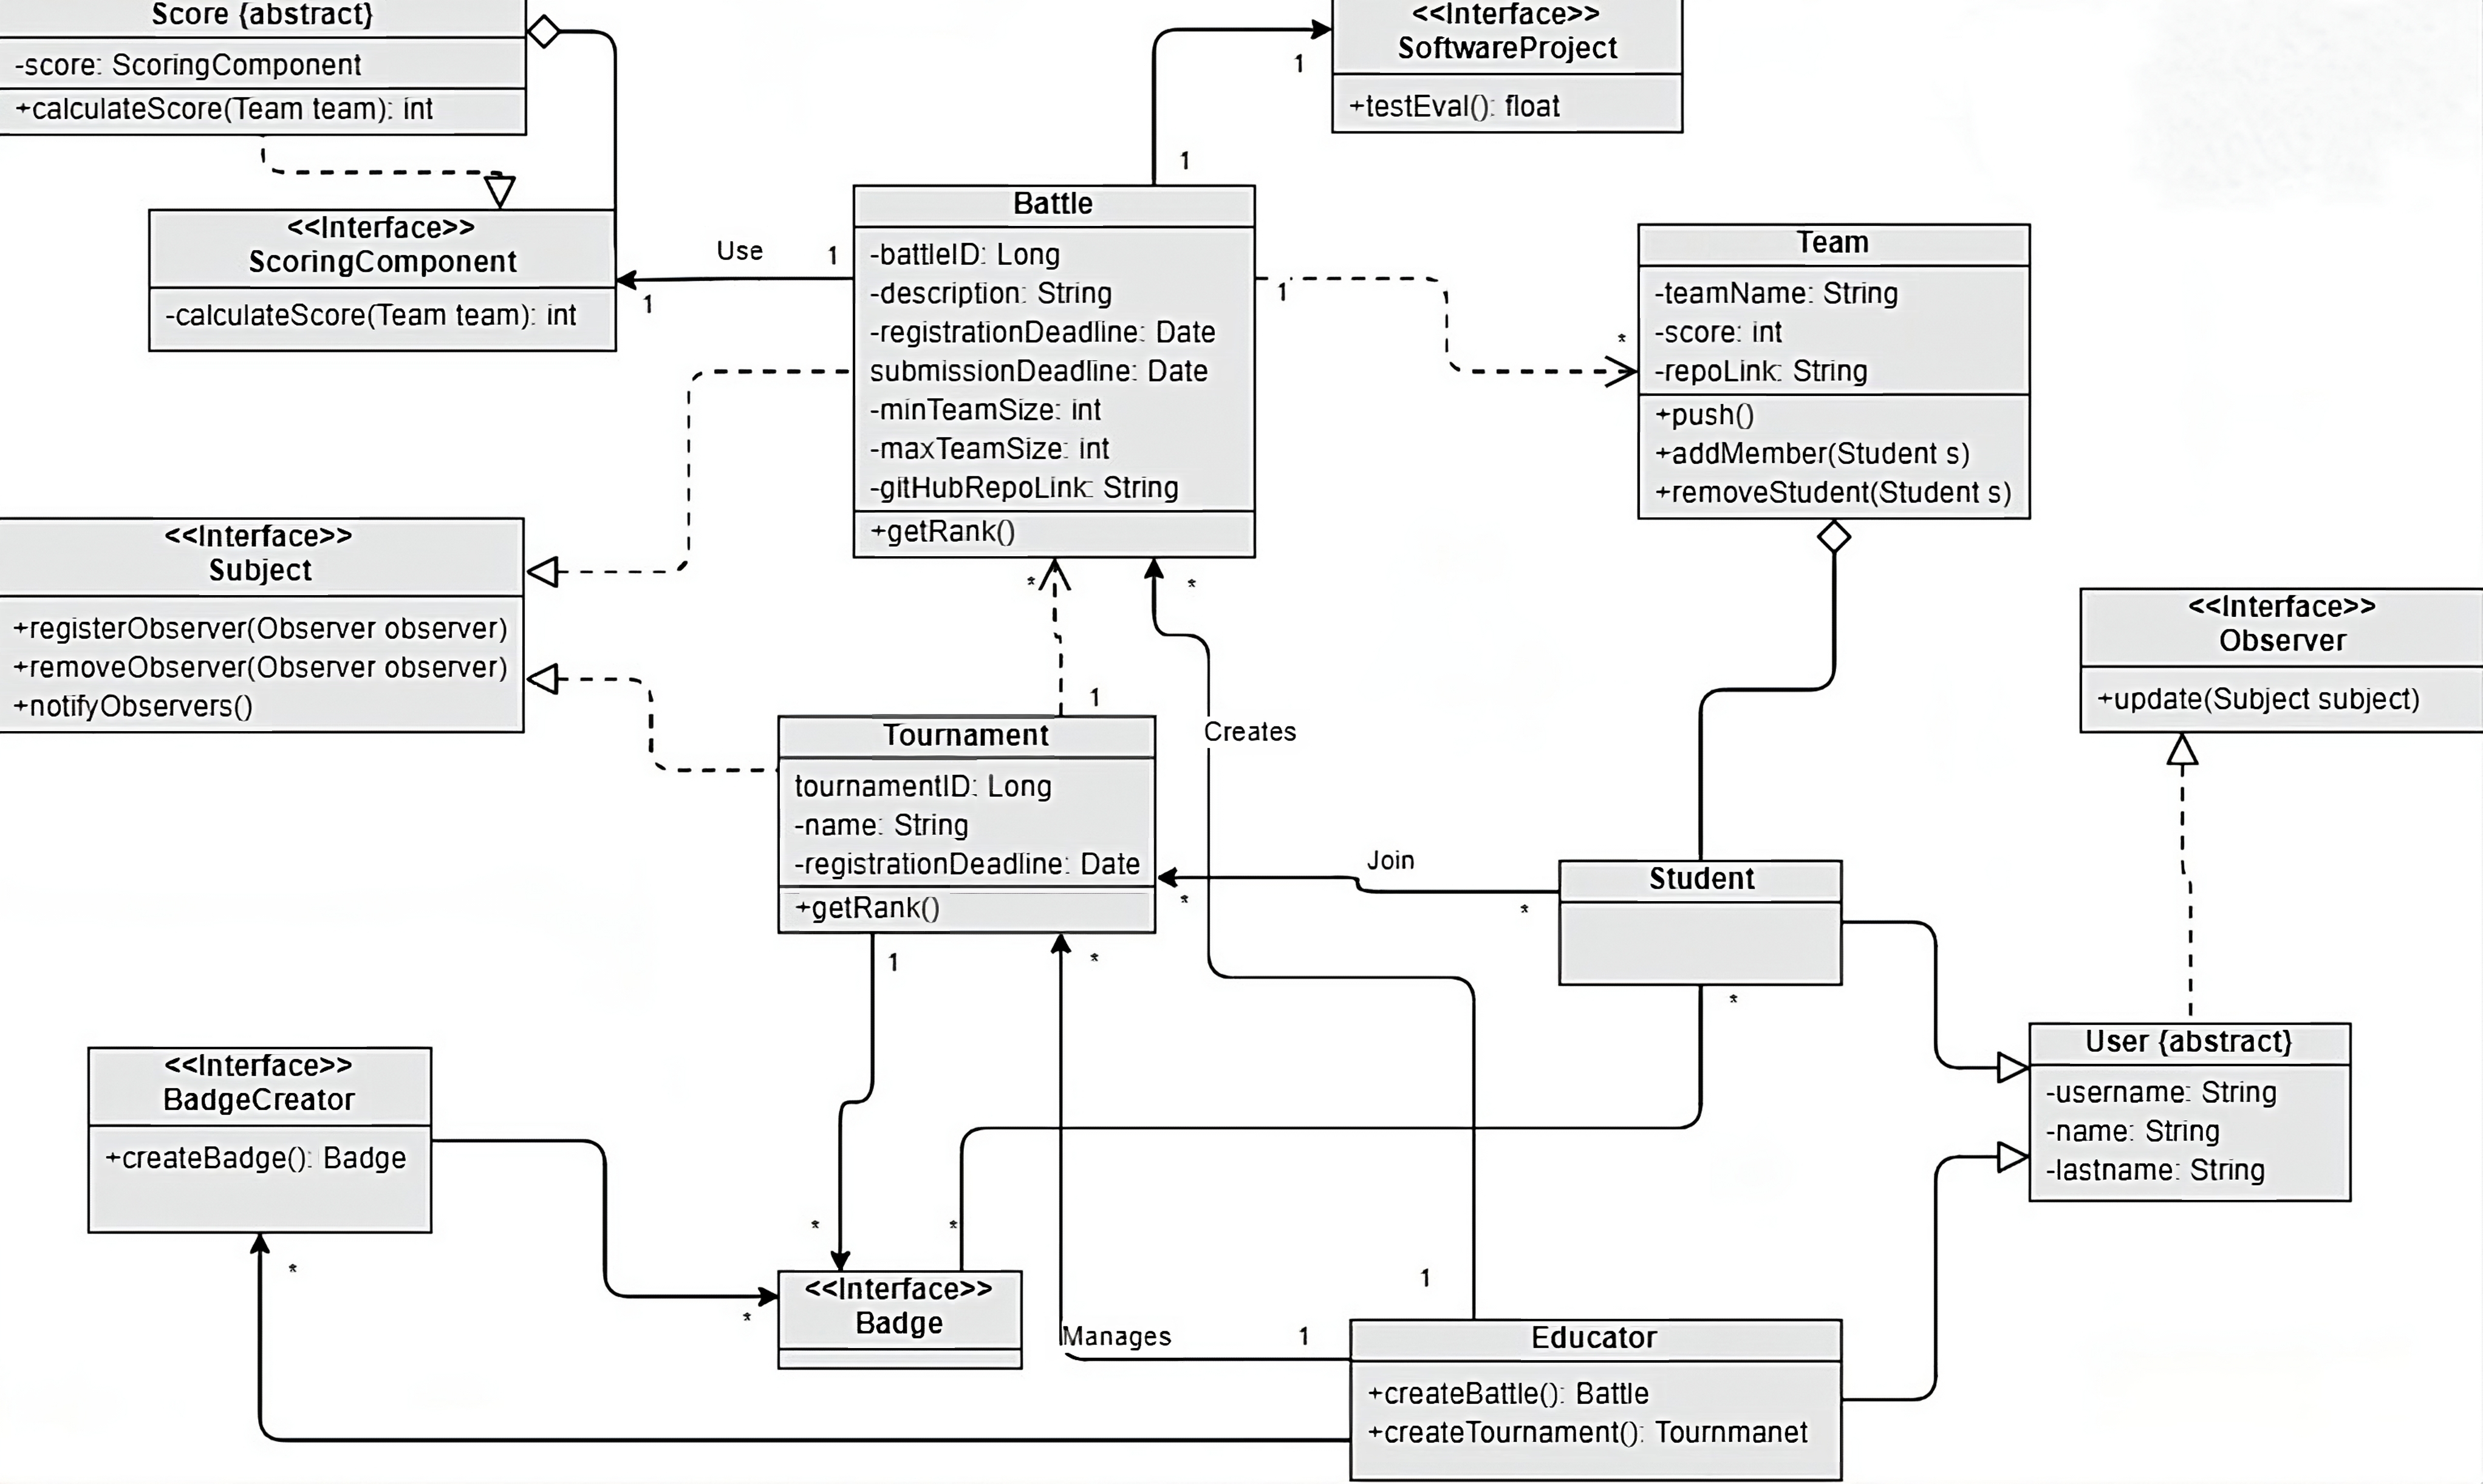
\includegraphics[width=0.9\linewidth]{Images/class-diagram.jpeg}
        \caption{A simplified Class Diagram}
        \label{fig:class_diagram}%
    \end{center}
\end{figure}